\documentclass{beamer}
\usetheme{Luebeck}
\usepackage{fontspec}
\beamertemplatenavigationsymbolsempty
\title{Something}
\author{Jack Rosenthal}
\date{26 October 2015}
\begin{document}

\begin{frame}
    \maketitle
\end{frame}

\begin{frame}
    \frametitle{Me}
    \pause
    \begin{itemize}
    \item I tell you to use Arch.\pause
    \item I won't read your emails if you send them in HTML.\pause
    \item I won't open your attachment if it is in a proprietary format. (ahem
        docx...)\pause
    \item Sometimes I won't even open your attachment even if it is in an open
        format.\pause
    \item I pay attention to little details like the kerning on fonts.\pause
    \item I switched keyboard layouts.\pause
    \item I switched twice more.\pause
    \item I made my own keyboard layout.\pause
    \item I made my own keyboard layout again.\pause
    \item I made yet another keyboard layout.\pause
    \item I built my own keyboard.\pause
    \item You probably would not be surprised if I was on a new keyboard layout
        tomorrow.\pause
    \item Therefore I will speak of keyboards.
    \end{itemize}
\end{frame}

\title{On Keyboards and Things...}

\begin{frame}
    \maketitle
\end{frame}

\begin{frame}
    \frametitle{A bit of history...}
    \pause
    The first keyboard layout was designed by the inventor of the
    typewriter, Christopher Latham Sholes. It looked a bit like a piano:\par
    \medskip
    \hskip30pt\texttt{- 3 5 7 9 N O P Q R S T U V W X Y Z}\par
    \hskip30pt\texttt{ 2 4 6 8 . A B C D E F G H I J K L M}

    \medskip
    \pause
    The problem with this is that bigrams like ST would jam the
    typewriter by slamming two bars near each other at once.

    \smallskip
    \pause
    Sholes fixed this by going through a trial and error process to eliminate
    the placement of common digraphs next to each other.

    \smallskip
    \pause
    The resulting layout looked like this:\par
    \begin{center}
    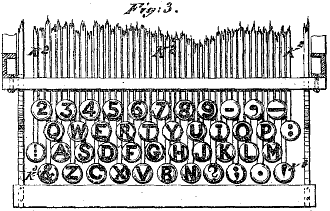
\includegraphics[width=3cm]{graphics/1878sholes}
    \end{center}
\end{frame}

\begin{frame}
    \frametitle{More history...}
    \begin{itemize}[<+->]
        \item Sholes sold his typewriter patent to Remington
        \item Remington sold a few hundred typewriters
        \item Sholes made a new typewriter without the clashing typebars,
            including a new efficient layout to go with it
        \item Remington liked his new typewriter, but did not want to change
            the QWERTY layout
        \item This made Sholes sad
        \item Sholes died of tuberculosis
    \end{itemize}
\end{frame}

\begin{frame}
    \frametitle{Issues with QWERTY}
    \begin{itemize}[<+->]
        \item Many common letter combinations require awkward finger motions.
        \item Many common letter combinations require a finger to jump over the home row.
        \item Many common letter combinations are typed with one hand. (e.g. was, were)
        \item Most typing is done with the left hand, which for most people is not the dominant hand.
        \item About 16\% of typing is done on the lower row, 52\% on the top
            row and only 32\% on the home row.
    \end{itemize}
\end{frame}

\begin{frame}
    \frametitle{Dvorak to the Rescue!}
    In 1932, Dr. August Dvorak and Dr. William Dealey designed a keyboard
    layout based off the concept of a \emph{home row}.
    \begin{center}
        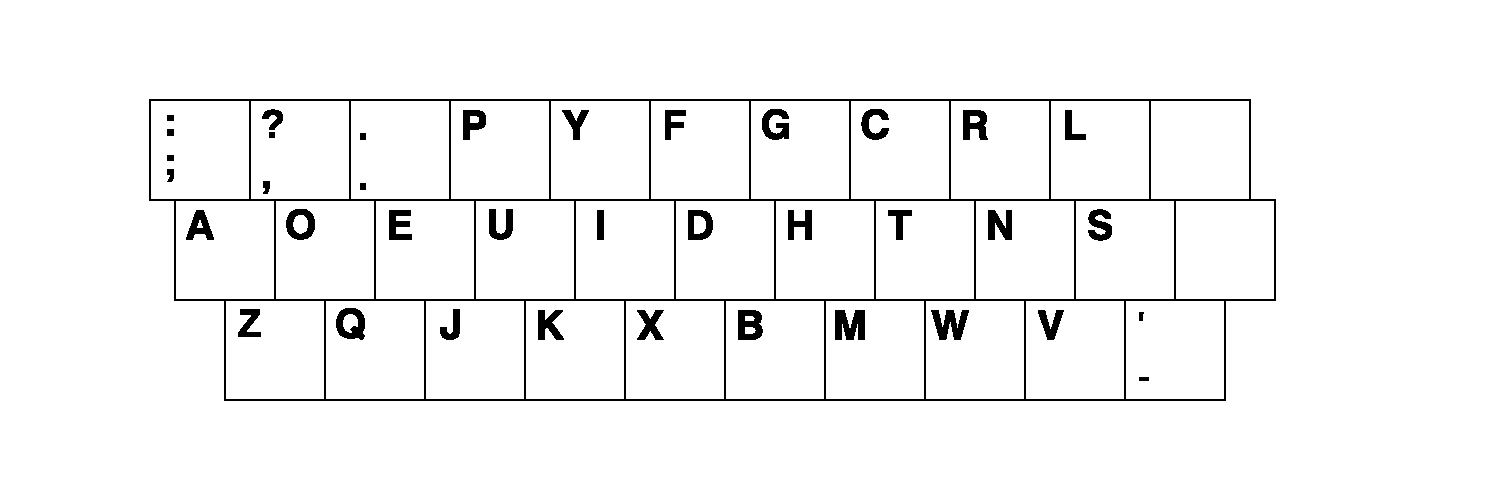
\includegraphics[width=\linewidth]{graphics/originaldvorak}
    \end{center}
\end{frame}

\begin{frame}
    \frametitle{Dvorak to the Rescue!}
    \begin{center}
    \vskip-1cm
        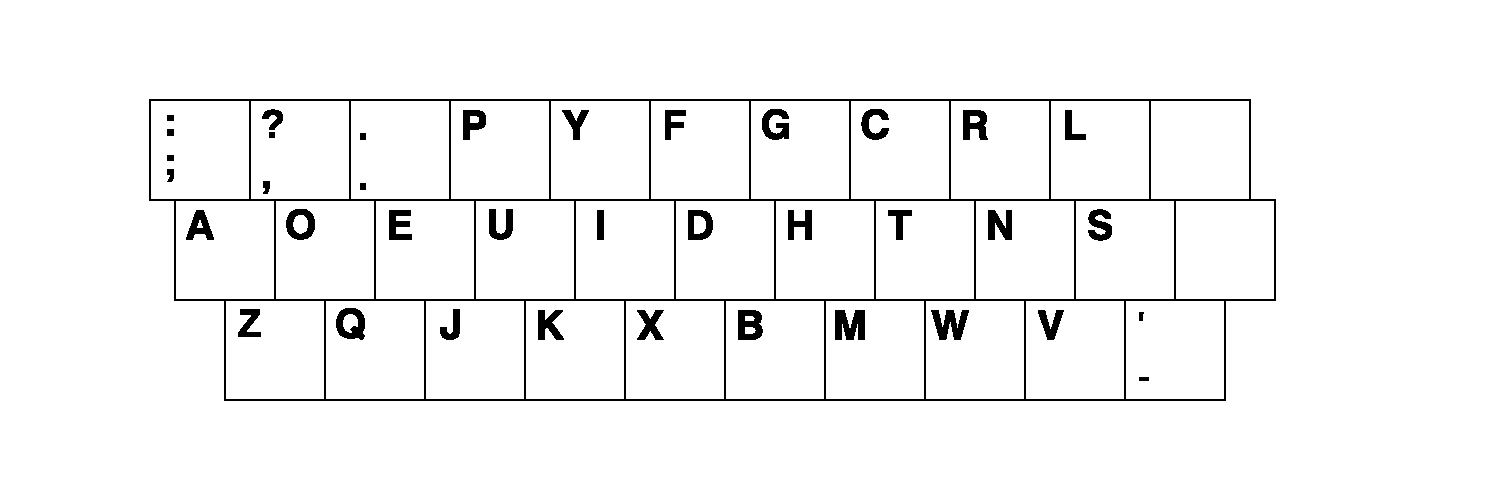
\includegraphics[width=\linewidth]{graphics/originaldvorak}
    \end{center}
    \vskip-1cm
    Dvorak and Dealey's design principles:
    \begin{itemize}[<+->]
        \item Letters should be typed by alternating between hands
            \begin{itemize}
                \item Vowels are on the left, consonants on the right
            \end{itemize}
        \item The most common letters and bigrams should be the easiest to
            type.
        \item The least common letters should be on the bottom row which is the
            hardest row to reach.
        \item The right hand should do more of the typing because most people
            are right-handed.
    \end{itemize}
\end{frame}

\begin{frame}
    \frametitle{Do your fingers hurt?}
    Typing \emph{Nineteen eighty-four} by George Orwell
    \begin{center}
        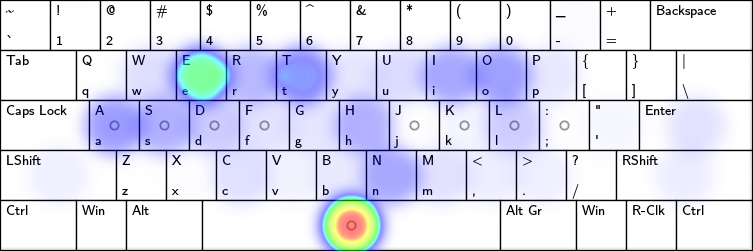
\includegraphics[width=0.8\linewidth]{graphics/qwertyheat}\par
        QWERTY: Distance fingers moved: 10.4 miles

        \smallskip
        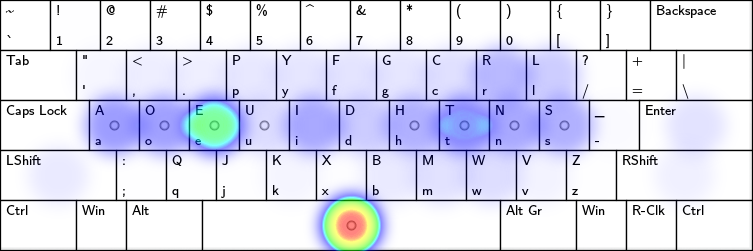
\includegraphics[width=0.8\linewidth]{graphics/dvorakheat}\par
        Dvorak: Distance fingers moved: 6.2 miles
    \end{center}
\end{frame}

\begin{frame}
    \frametitle{Why did I initially switch keyboard layouts?}
    \pause
    \begin{itemize}[<+->]
        \item Jessie Weaver is entirely responsible for this.
        \item But he led me to do my own research.
    \end{itemize}
\end{frame}

\begin{frame}
    \frametitle{Colemak}
    \begin{center}
        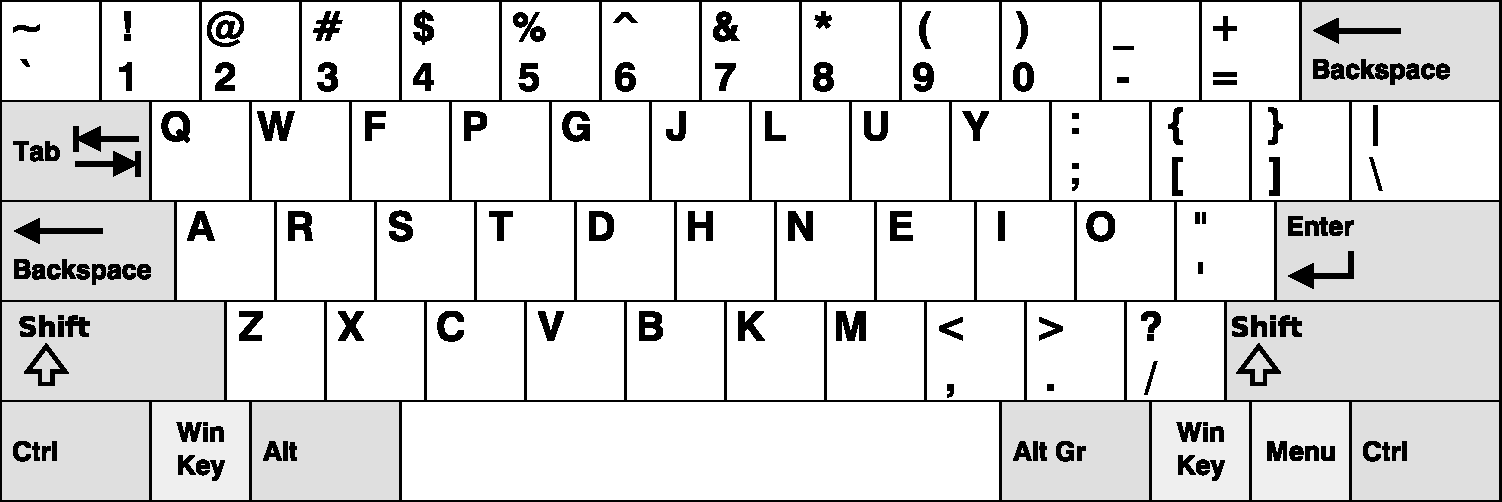
\includegraphics[width=0.8\linewidth]{graphics/colemak}\par
    \end{center}
    \pause
    Design principles:
    \begin{itemize}
        \item Change QWERTY as little as possible while bringing efficency
            simmilar to Dvorak.
        \item Be easy to learn if you are already a good QWERTY typist.
    \end{itemize}
    \pause
    Why I abandoned it:
    \begin{itemize}
        \item It's no better at programming than QWERTY.
        \item It dosen't have enough hand alternation for my liking.
        \item Too much lateral motion while typing.
    \end{itemize}
\end{frame}

\begin{frame}
    \frametitle{Colemak: Heat Map}
    Typing \emph{Nineteen eighty-four} by George Orwell
    \begin{center}
        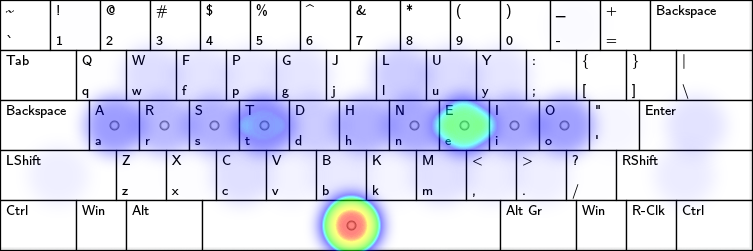
\includegraphics[width=\linewidth]{graphics/colemakheat}\par
    Distance fingers moved: 5.9 miles
    \end{center}
\end{frame}

\begin{frame}
    \frametitle{Antibracket}
    A keyboard layout designed to combine the ambition of Dvorak, practicality
    of Colemak, and the symbols of Neo.
    \begin{center}
        \only<1,4>{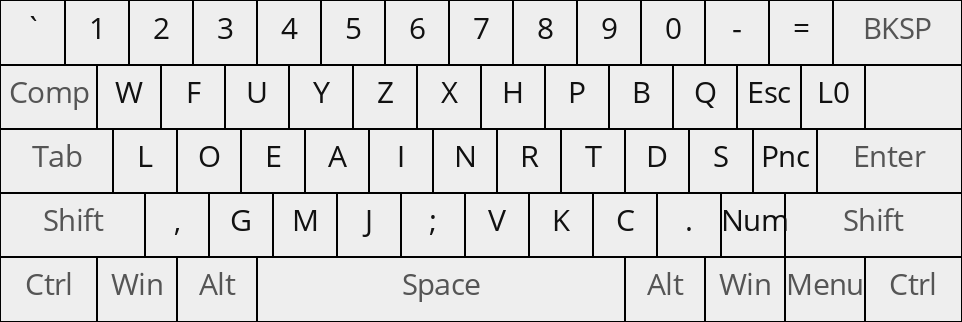
\includegraphics[width=0.8\linewidth]{graphics/abmain}}
        \only<2>{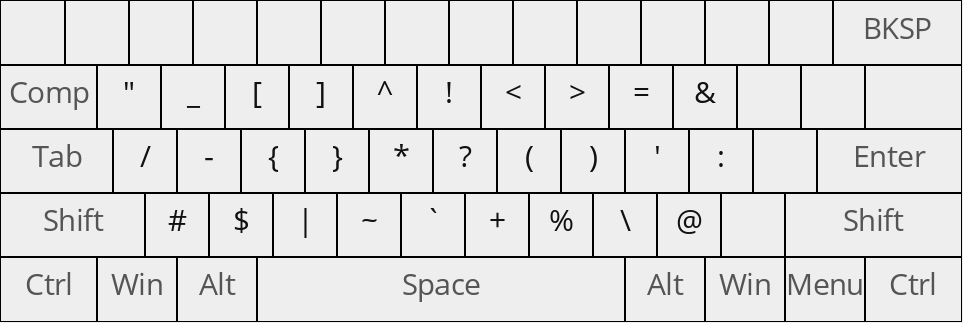
\includegraphics[width=0.8\linewidth]{graphics/absym}}
        \only<3>{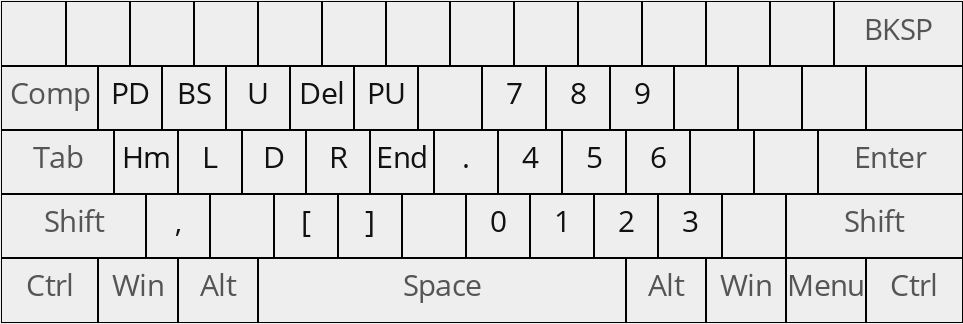
\includegraphics[width=0.8\linewidth]{graphics/abnum}}
    \end{center}
    \visible<4>{
    Why I abandoned it:
    \begin{itemize}
        \item I already knew how to type in Colemak and was lazy.
    \end{itemize}
}
\end{frame}

\begin{frame}
    \frametitle{Antibracket: Heat Map}
    Typing \emph{Nineteen eighty-four} by George Orwell
    \begin{center}
        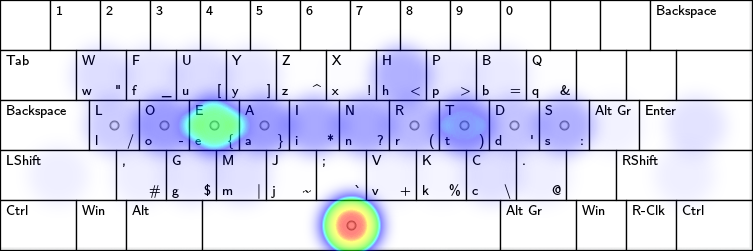
\includegraphics[width=\linewidth]{graphics/abheat}\par
    Distance fingers moved: 6.3 miles
    \end{center}
\end{frame}

\begin{frame}
    \frametitle{The WULY Antimak}
    \begin{block}{Me on 13 Feb 2015}
        An ergonomic modifier based keyboard layout with Antibracket's symbols and numbers and a home row practically stolen from Colemak. Also focuses around ease of vimming and still optimised for the English language... so basically it's crack for your keyboard.
    \end{block}
    \begin{center}
        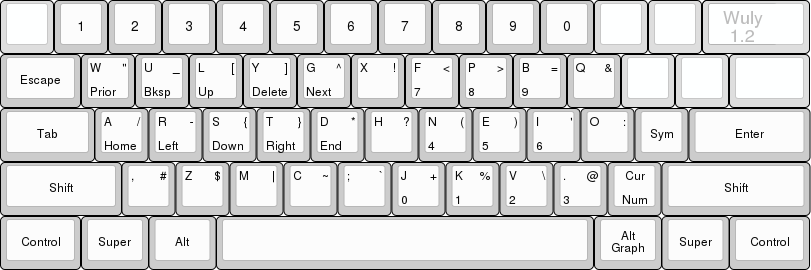
\includegraphics[width=\linewidth]{graphics/wuly}
    \end{center}
\end{frame}

\begin{frame}
    \frametitle{WULY: Heat Map}
    Typing \emph{Nineteen eighty-four} by George Orwell
    \begin{center}
        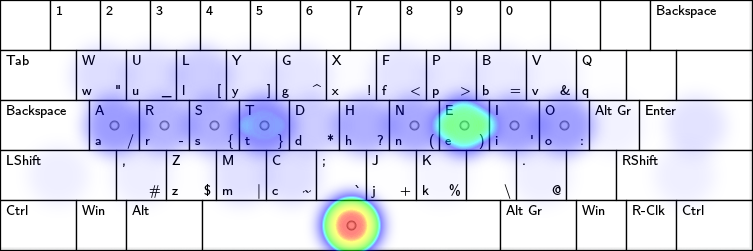
\includegraphics[width=\linewidth]{graphics/wulyheat}\par
    Distance fingers moved: 5.6 miles
    \end{center}
\end{frame}

\begin{frame}
    \frametitle{My BuTeck ADNW Variant}
    \begin{center}
        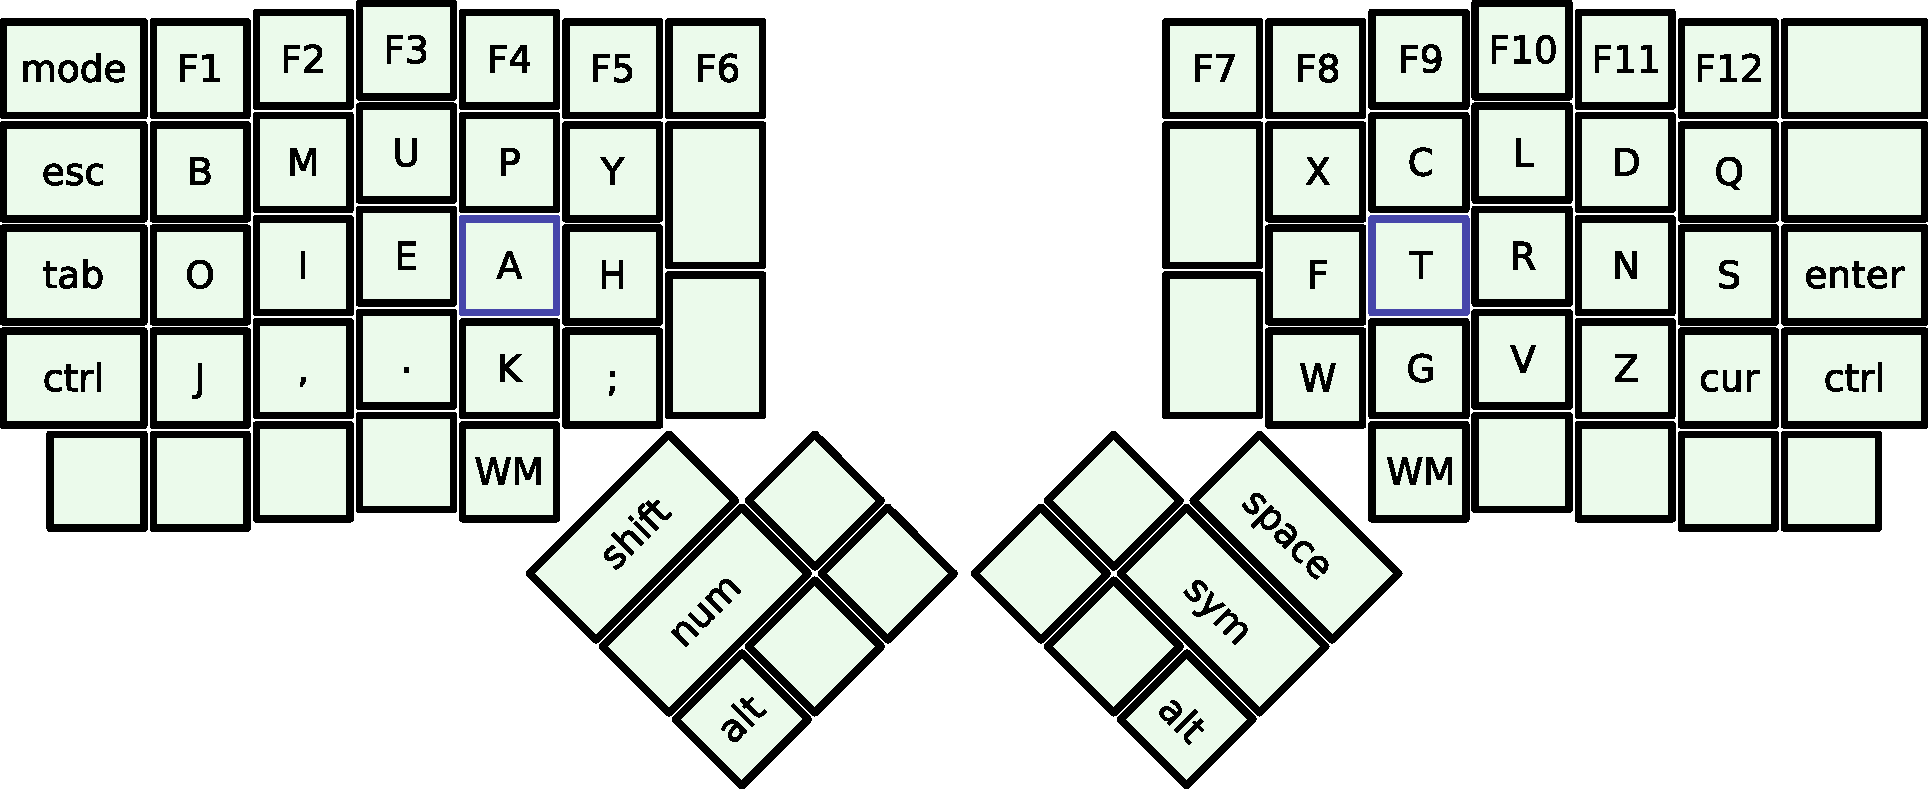
\includegraphics[width=\linewidth]{graphics/doxicalmain}
    \end{center}
\end{frame}

\begin{frame}
    \frametitle{Jack's Third Layout: Three}
    \begin{center}
        \only<1>{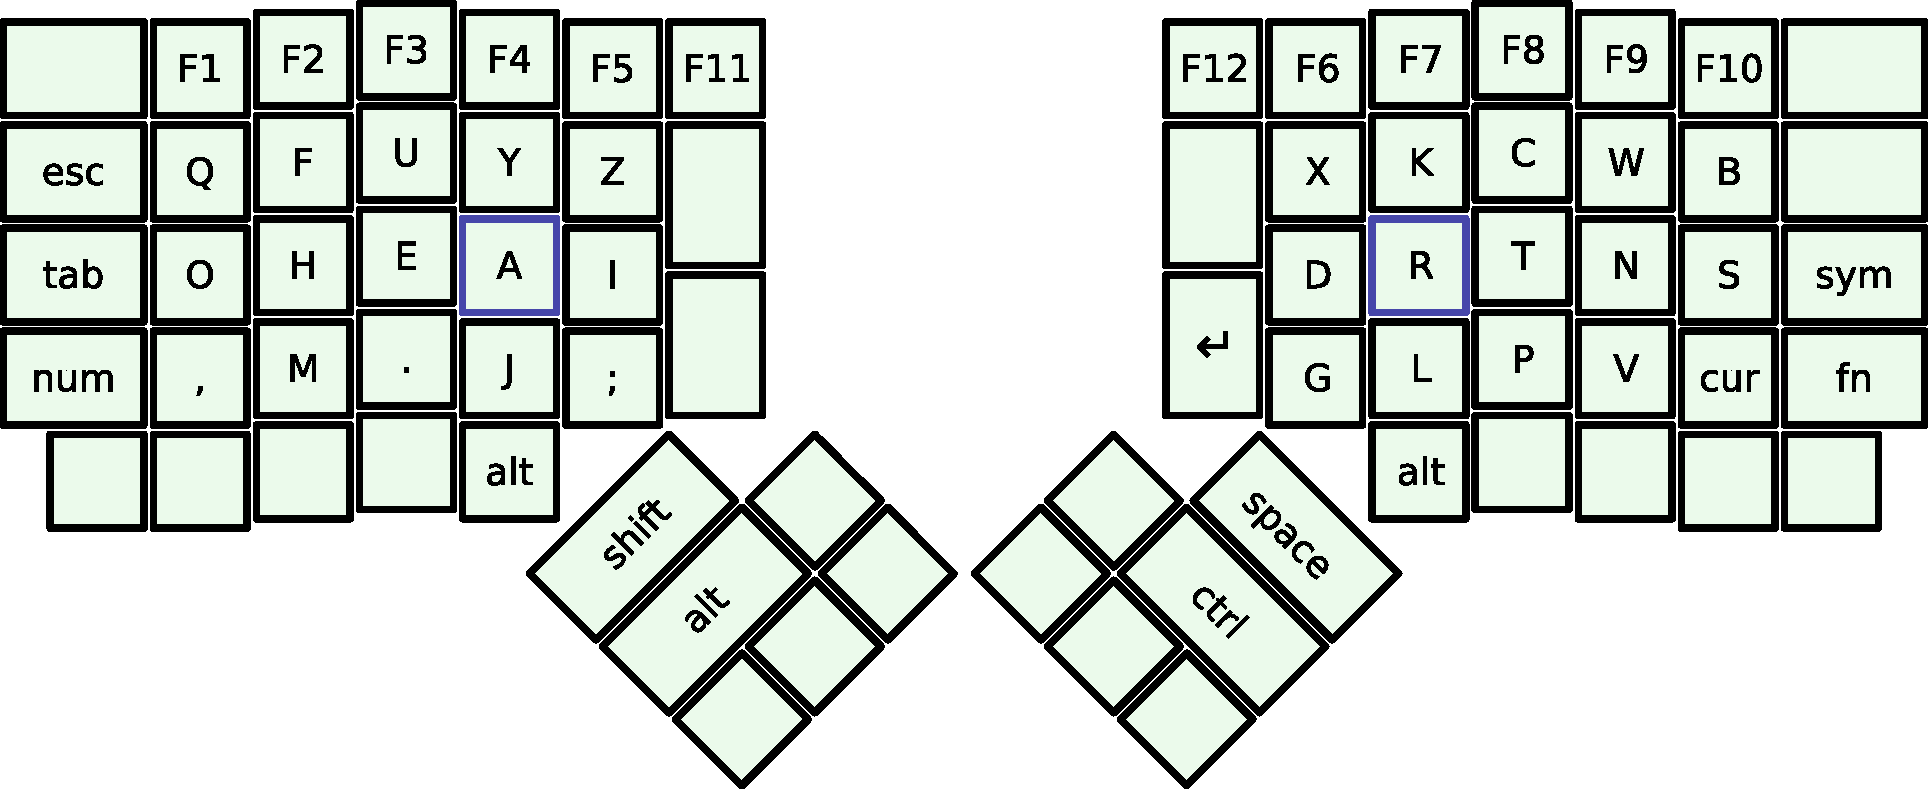
\includegraphics[width=\linewidth]{graphics/three}}
        \only<2>{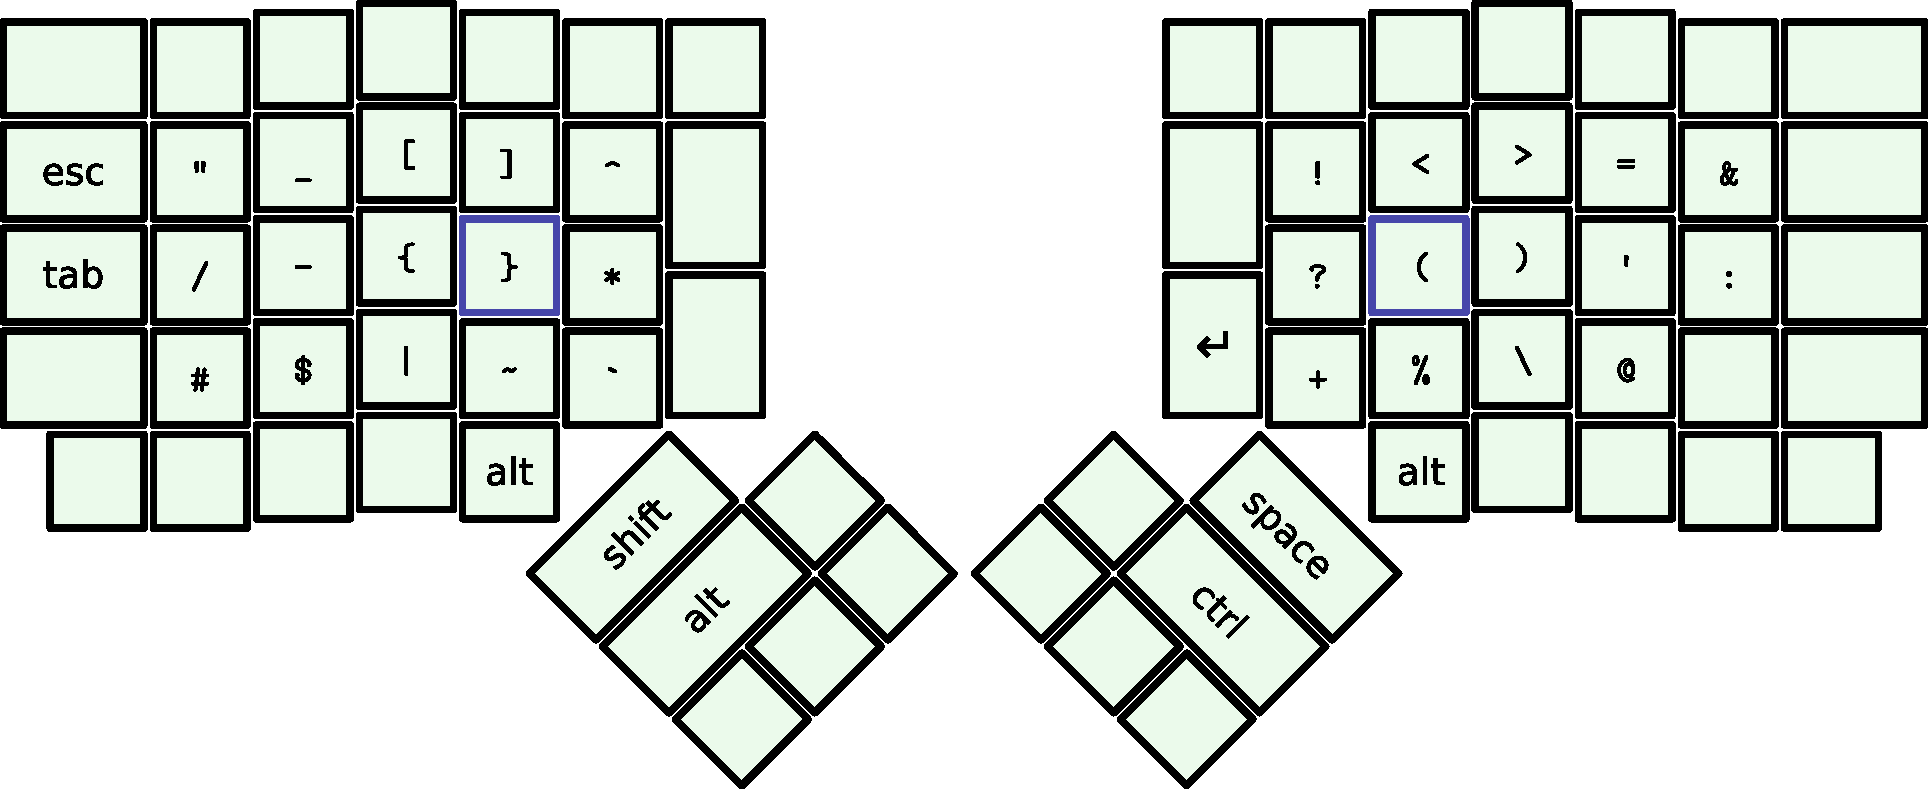
\includegraphics[width=\linewidth]{graphics/threesym}}
        \only<3>{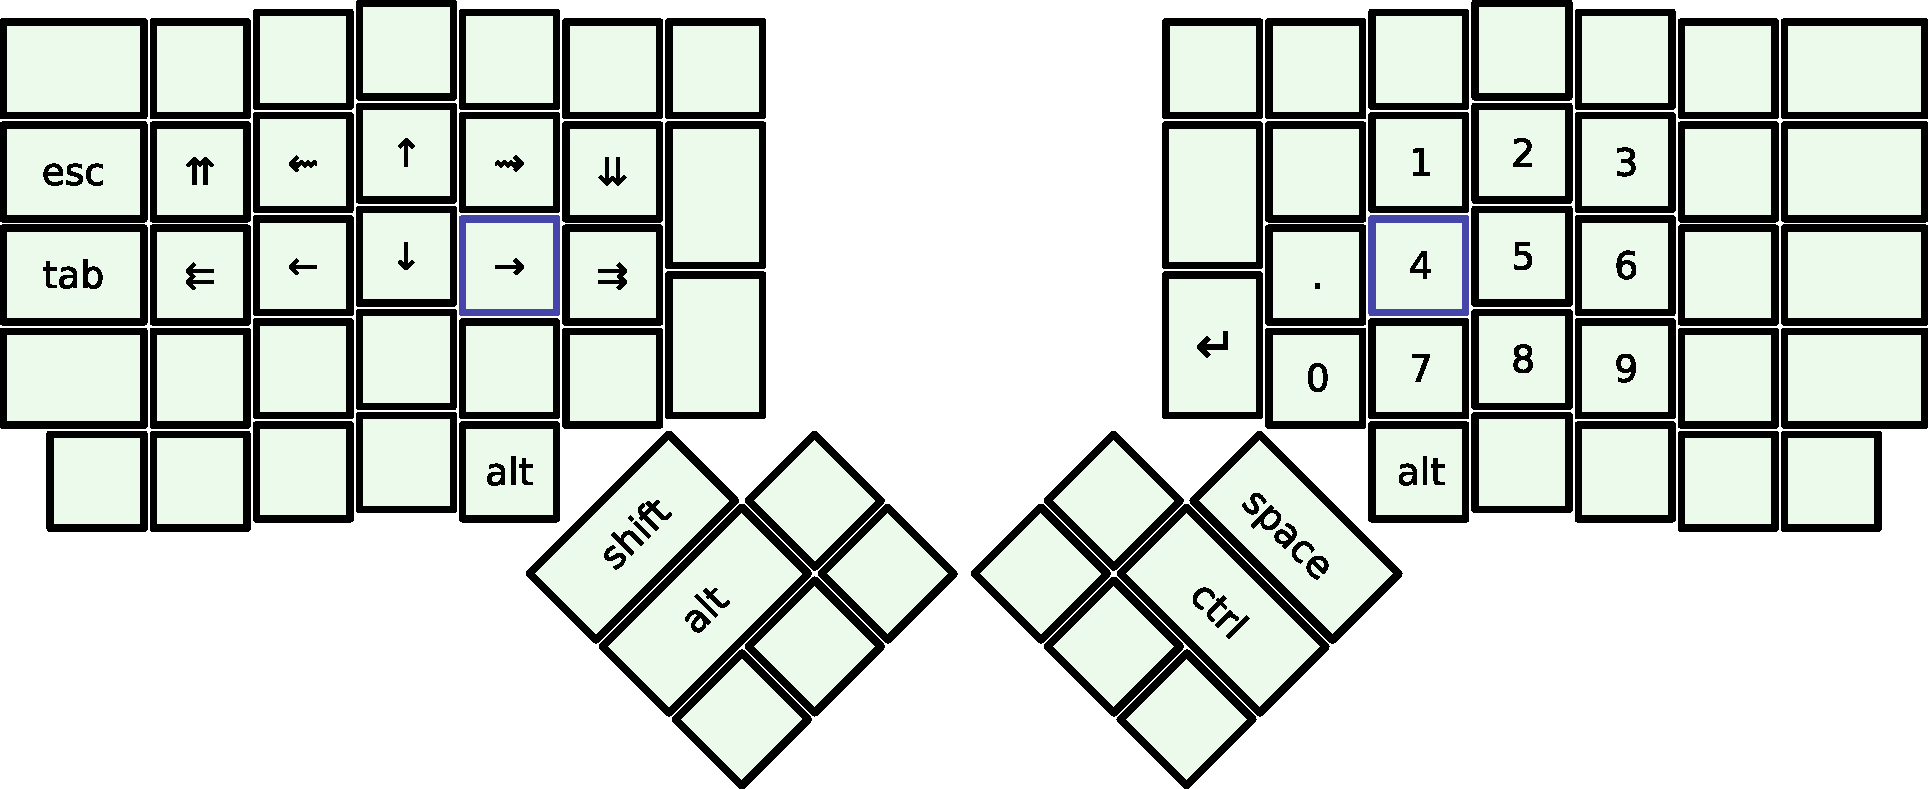
\includegraphics[width=\linewidth]{graphics/threenum}}
    \end{center}
\end{frame}

\begin{frame}
    \frametitle{Three: Heatmap}
    Typing \emph{Nineteen eighty-four} by George Orwell
    \begin{center}
        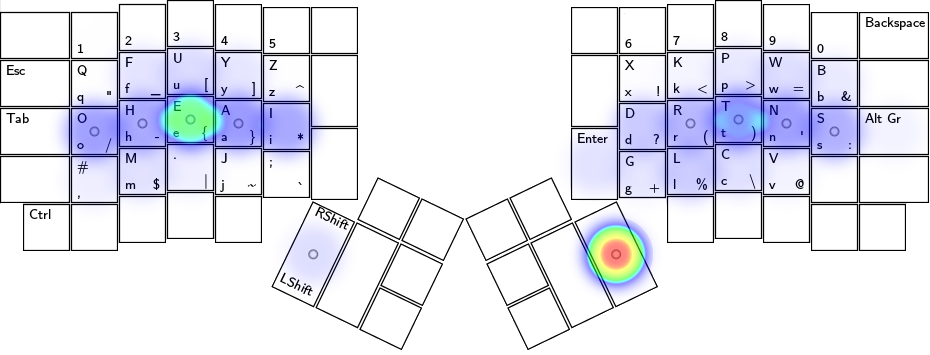
\includegraphics[width=\linewidth]{graphics/threeheat}\par
    Distance fingers moved: 4.9 miles
    \end{center}
\end{frame}

\begin{frame}
    \frametitle{Other notable keyboard layouts worth researching}
    \begin{itemize}[<+->]
        \item Programmers Dvorak
        \item Workman
        \item ARENSITO
        \item LCK (Ask Jason)
        \item Neo
        \item ADNW
        \item BuTeck ADNW
    \end{itemize}
\end{frame}

\begin{frame}
    \frametitle{Switching keyboard layouts}
    \begin{enumerate}[<+->]
        \item Print out the layout reference card and prop it up in front of
            your monitor.
        \item Change layouts on your computer. Don't rearrange your keys to
            match your layout.
        \item Throw out the reference card after you know where everything is.
            This should be after a few hours of use.
        \item Struggle. You must go cold turkey for the switch to be effective.
        \item Keep struggling. Focus on accuracy, not speed.
        \item Once you are accurate, you will naturally start to type faster.
        \item Impress your friends.
    \end{enumerate}
\end{frame}

\begin{frame}
    \frametitle{You}
    \begin{itemize}[<+->]
        \item If you use QWERTY, don't.
        \item You should do your own research and find a keyboard layout you
            like.
        \item There is no best keyboard layout, each layout has it's
            advantages.
    \end{itemize}
\end{frame}

\end{document}
